\chapter{网络流量特征分析和特征重要度评估}{
{
\let\cleardoublepage\relax
}
\label{chap:analyze}

针对基于网络流量的横向移动检测,本文研究和分析了横向移动的原理及其在容器化环境中的行为,以及这些横向移动行为在网络流量特征中的表现。随后,本文对特征进行了最值分析和密度分析,然后进行特征重要度评估。通过这些分析,本文发现对于少量关键的横向移动流量,可进行最值判别;对于大多数横向移动流量,可进行特征筛选,为此,本文进行了特征的重要度评估并进行排序,其评估结果可用于后续模型的训练和测试工作。

\section{横向移动原理分析}
\label{sec:theory}

\subsection{横向移动总体过程}

当攻击者成功进入到目标网络的初始入侵点之后,他往往需要继续访问其初始入侵点以外的其他机器,这是因为他们的主要目标往往不在初始入侵点之上。他们需要继续探索网络以找到他们的目标,然后获得对目标的访问权限。为了达到他们的目标,攻击者可能会安装自己的远程访问工具以控制初始入侵点。

在企业网络中,用户需要使用其凭据才能登录到计算机。然而,攻击者的初始入侵点和主要目标往往不在同一台计算机上,为了达到目标,他们需要切换多个凭据。Hopper \citep{ho2021hopper} 正是利用了这一点,提出了基于凭据切换检验的横向移动检测方法。其他工作 \citep{king2023euler, khoury2023jbeil} 则是基于这些凭据的认证记录,以用户、计算机为节点,凭据认证记录为边,建立动态图模型,以检测横向移动行为。

在移动终端上,攻击者则利用远程服务或串行总线(Universal Serial Bus,USB)来移动到其他设备\citep{mitre2024lm}。例如,攻击者可以使用虚拟专用网(Virtual Private Network,VPN)连接到远程服务,当该服务存在漏洞或后门时,就有可能成功被攻击者利用;攻击者还可以将恶意软件通过 USB 传输并安装到其他计算机上,从而完成一次横向移动操作。

在工业控制系统(Industrial Control Systems,ICS)中,攻击者则可以使用设备中的默认凭据或硬编码凭据、漏洞利用等方式来实施横向移动\citep{mitre2024ics}。

虽然横向移动在不同的环境之下所采用的具体技术不同,但是其共同之处在于攻击者利用这些技术,从当前入侵点访问下一台目标机器。在这些环境中,企业网络环境由于包含了用户的凭据信息,因此为横向移动的检测提供了宝贵的信息,大多数关于横向移动检测的研究工作均在企业网络环境下进行。

\subsection{容器化集群的组件}

在容器化环境中,横向移动的过程包括从对一个容器的给定访问权限获取对集群中各种资源的访问权限,或从容器获取对底层主机的访问权限,或获取对云环境的访问权限。因此,这与容器化集群的组件息息相关。容器化集群的组件如图~\ref{fig:cluster}~所示\citep{k8scomp}。

\begin{figure}[t]
    \centering
    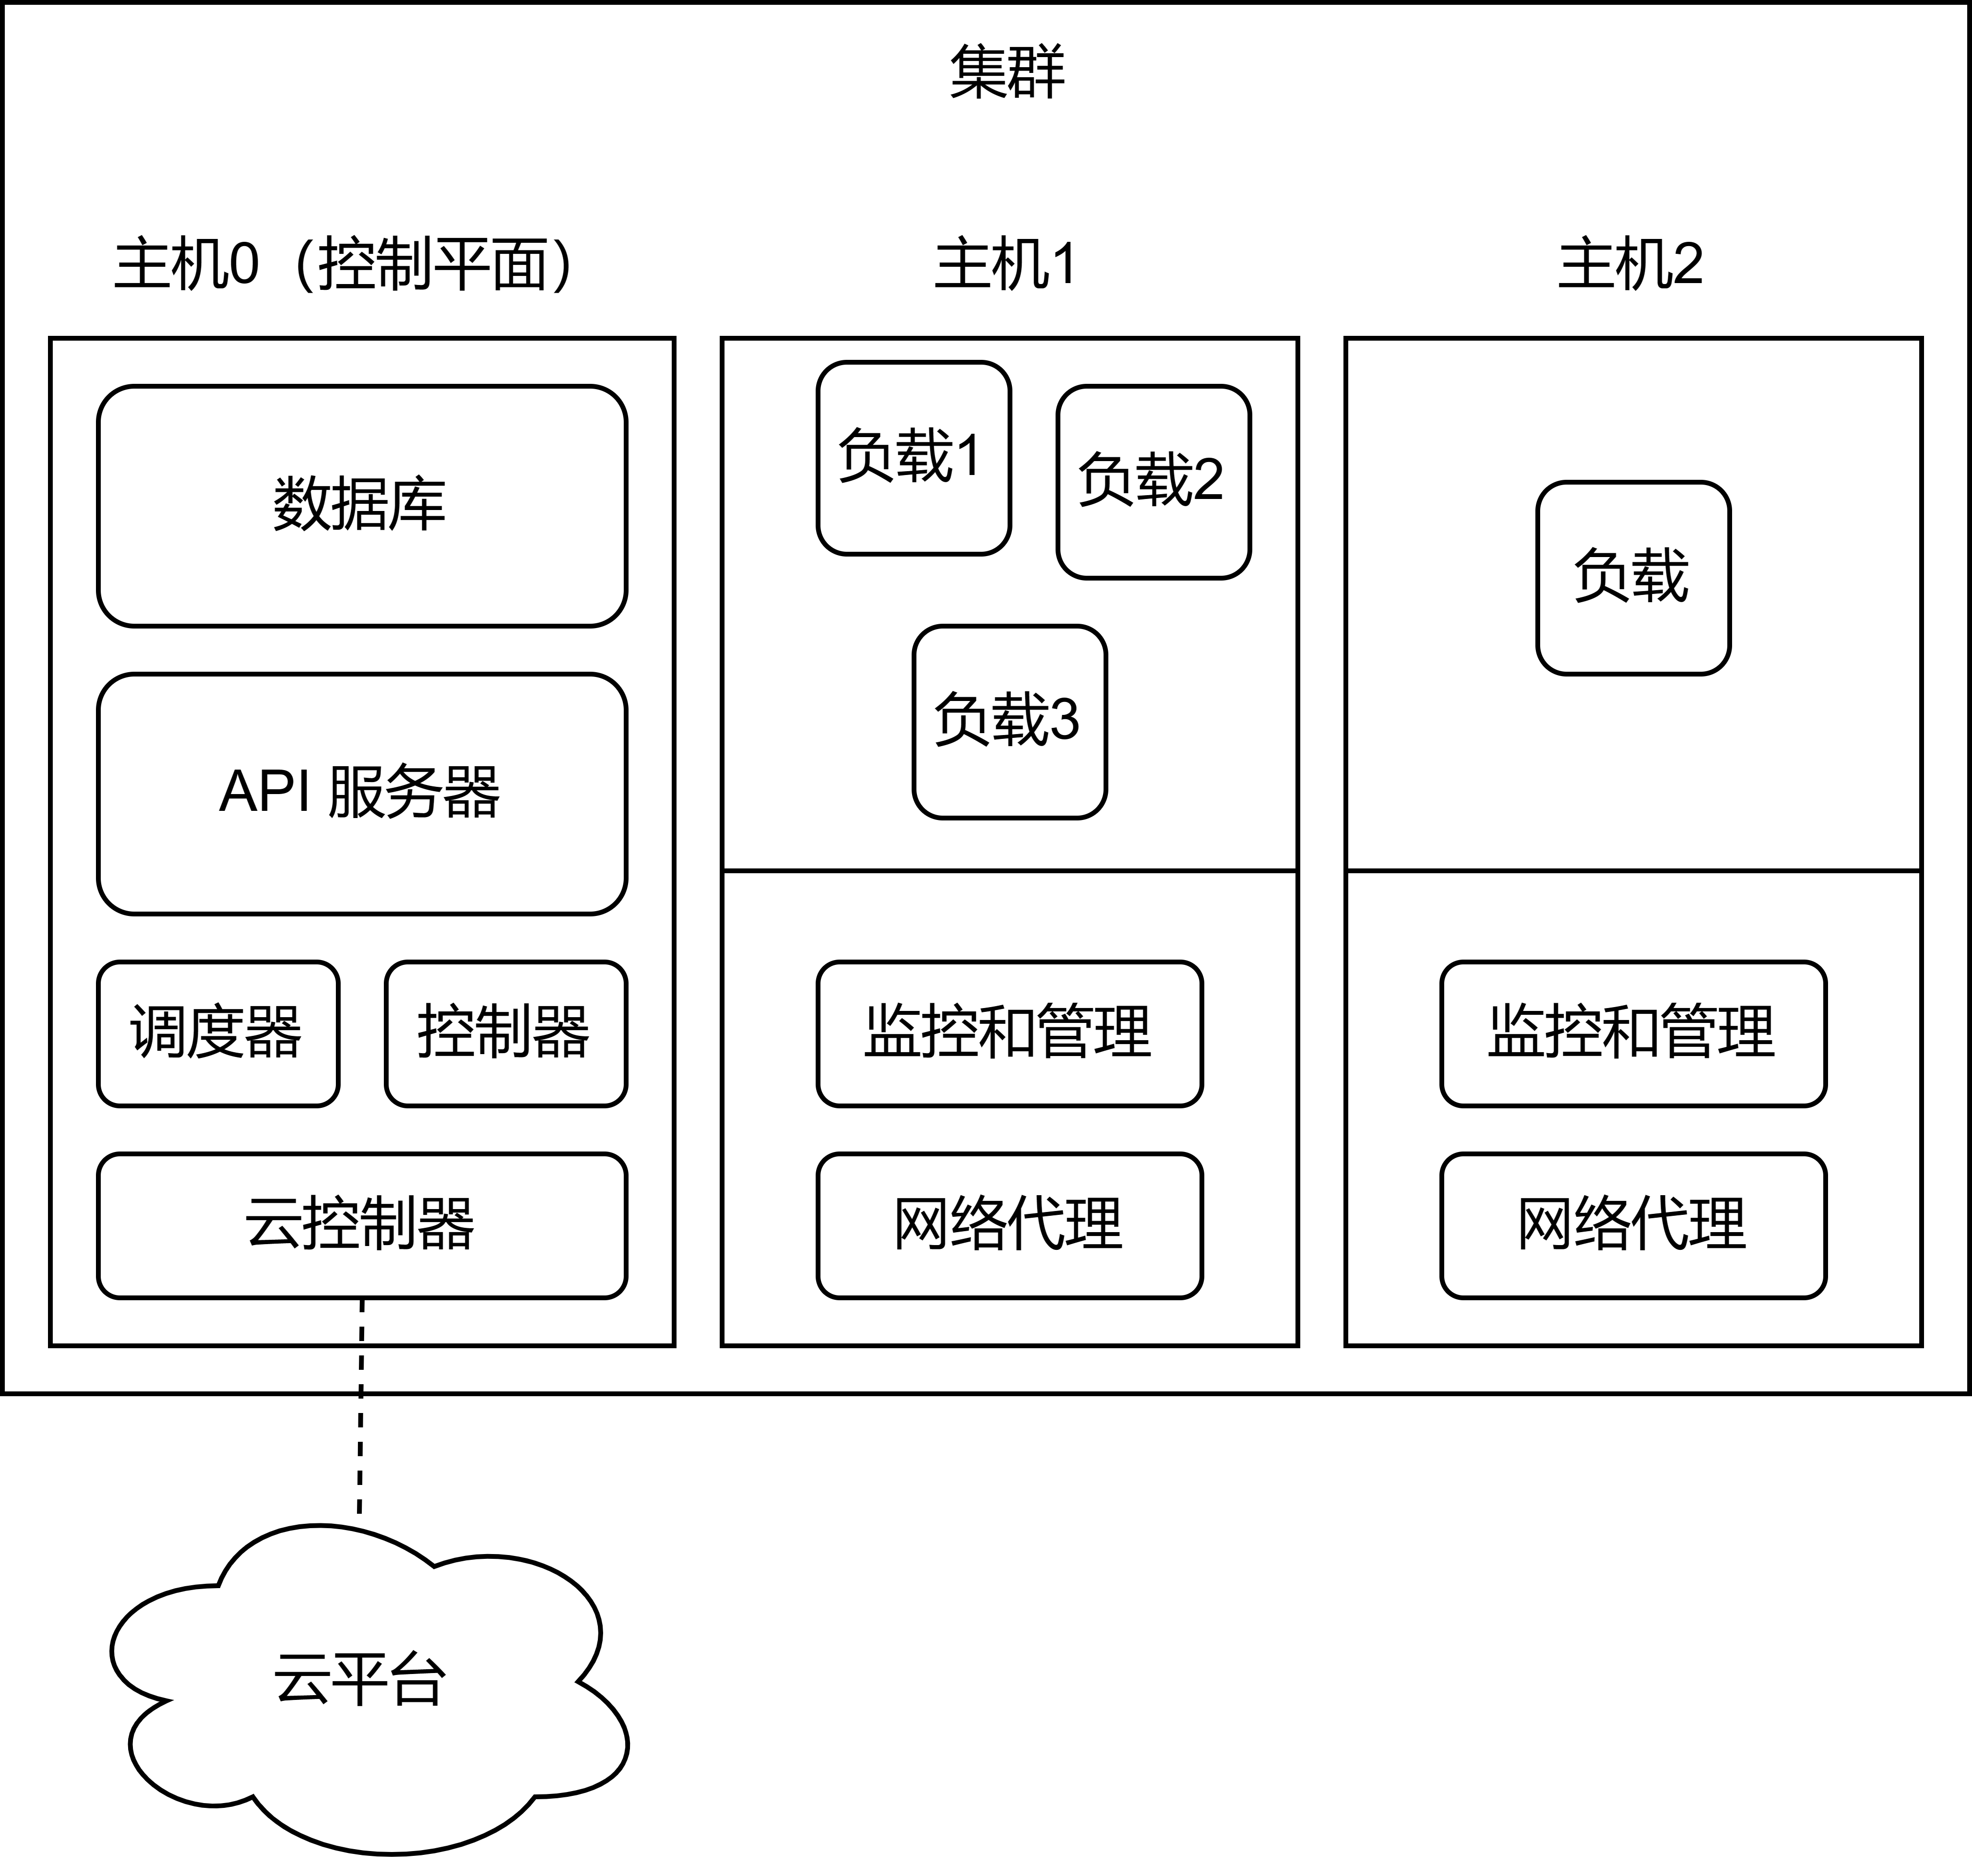
\includegraphics[width=0.7\textwidth]{cluster}
    \bicaption{\enspace 容器化集群组件}{\enspace The components of a containerized cluster}
    \label{fig:cluster}

\end{figure}

容器化集群由若干个主机组成,一般由其中一台主机集中部署控制平面组件,包括 API 服务器、数据库、调度器、控制器、云控制器等;其他主机部署应用程序负载。

在控制平面中,数据库存放集群数据,例如应用程序凭据、云平台的凭据等。API 服务器是控制平面的前端,负责接受请求并处理。调度器负责将应用程序负载调度到集群中的主机上运行。控制器负责处理主机异常时的通知和响应等。云控制器则负责与云平台对接,以便用户通过云平台的仪表板控制容器化集群,并在仪表板上展示容器化集群的状态。

在控制平面以外的主机上运行着多个负载,每个负载包括多个容器。

在容器化集群中,为了实现负载均衡并提高应用程序的可用性,一个应用程序通常对应二个或以上的负载,这些负载共同组成一个对外提供的服务。容器化集群中的服务、负载和主机之间的网络结构如图~\ref{fig:networking}~所示 \citep{k8snet}。

\begin{figure}[t]
    \centering
    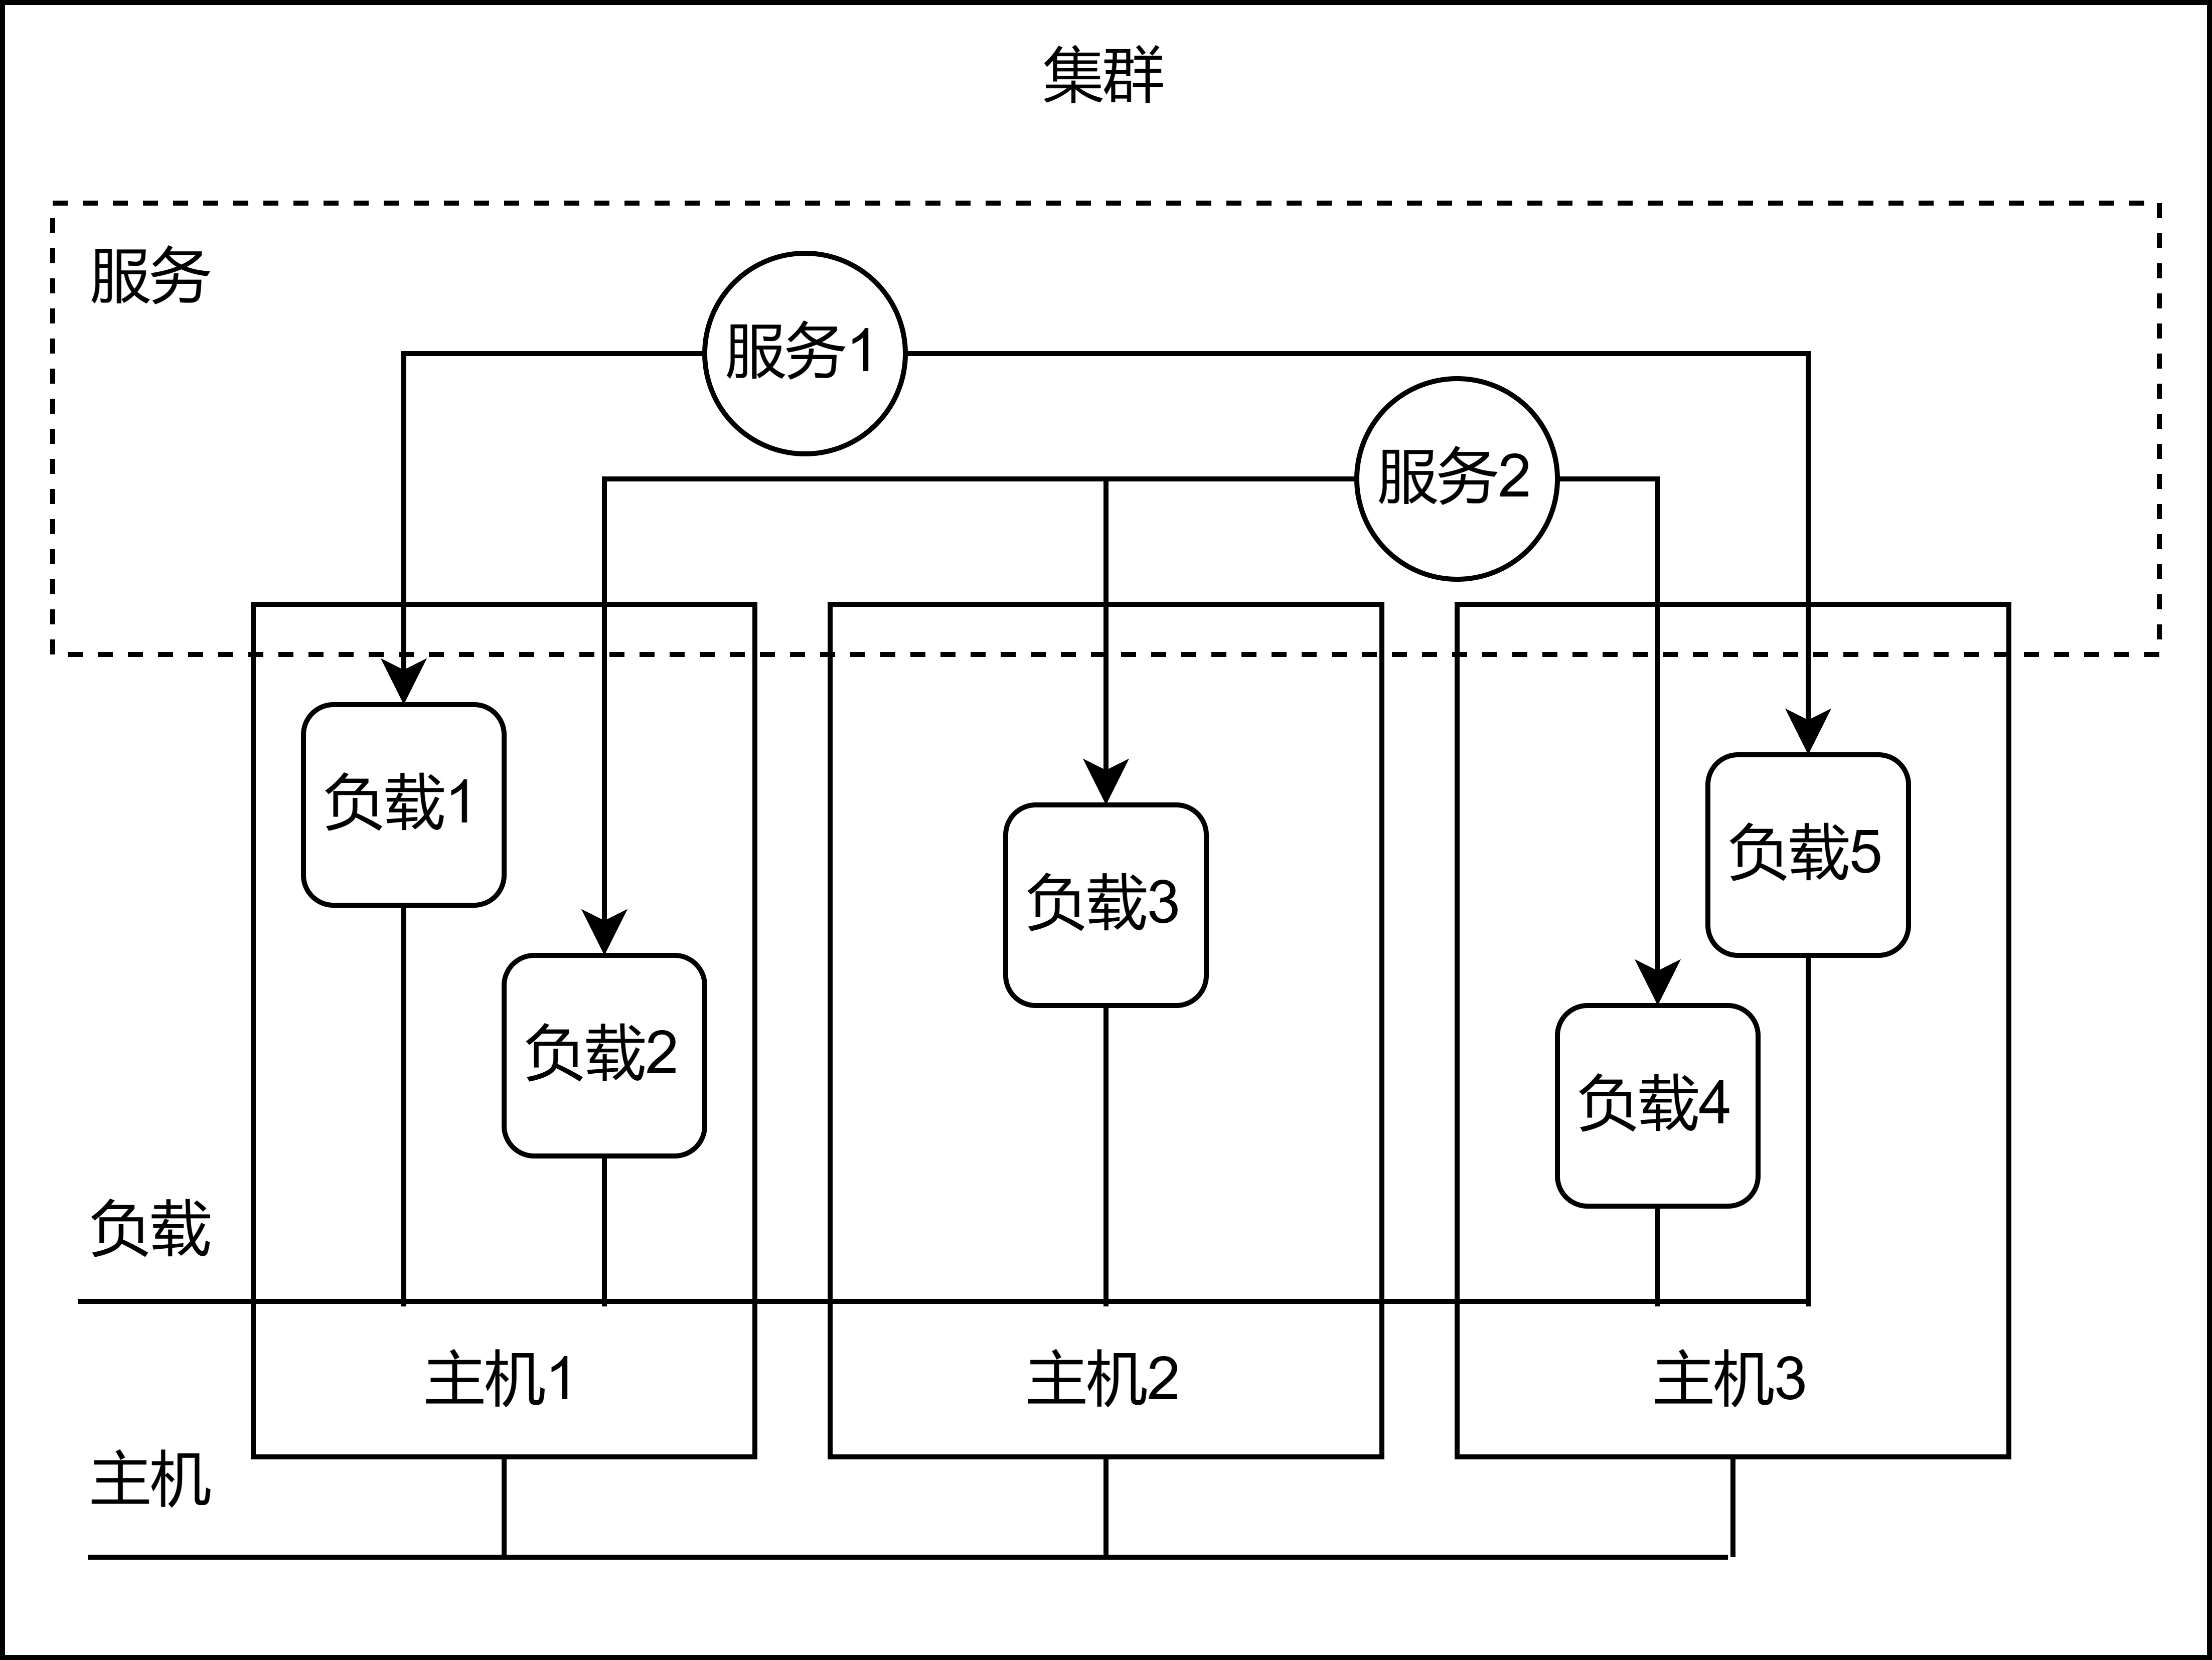
\includegraphics[width=0.80\textwidth]{networking}
    \bicaption{\enspace 容器化集群网络结构}{\enspace The networking architecture of a containerized cluster}
    \label{fig:networking}

\end{figure}

在容器化集群中,API 服务器向集群中的服务分配 IP 地址;不同的负载之间处于同一个网段内,可以直接通过 IP 地址互相访问,由集群的网络插件分配 IP 地址;不同的主机通常配置在同一个网段内,若集群通过云平台部署,则由云控制器分配 IP 地址。

\subsection{容器化集群中的横向移动}

容器化集群的结构为横向移动提供了可能,包括以下行为 \citep{yossi2020threat}:

\begin{itemize}
    \item {从集群移动到云平台:攻击者侵入负载后,利用挂载到负载当中的凭据,非法访问云平台。}
    \item {在负载之间移动:由于容器化集群中的各个负载处于同一个网段内,并在默认情况下允许互相访问,因此攻击者在侵入到其中一个负载之后,可能会非法访问另一个负载。}
    \item {非法请求资源:容器化环境中的负载默认挂载了相应的服务账户凭据。当攻击者侵入负载后,他可以利用该凭据向 API 服务器发起非法请求,以获取集群中的配置文件和其他资源。}
    \item {从负载移动到主机:当上述服务账户具有创建新容器的权限时,攻击者可以创建一个新负载并将主机上的目录挂载到该负载中,从而非法控制主机;也可通过容器逃逸漏洞来控制主机。}
\end{itemize}



% 在容器化集群中,API 服务器作为控制平面的前端,负责处理身份验证和鉴权,工作负载、服务、配置文件等的增、删、改、查操作,既影响集群的行为,也影响集群数据库中存储的敏感信息的机密性、完整性。在上述横向移动行为中,除在负载之间移动以外,其他行为均需和 API 服务器通信;在负载之间的移动虽然不直接与 API 服务器通信,但需要查询集群中的负载情况,此时需要和 API 服务器通信。因此,对 API 服务器相关流量的检测是横向移动检测的重点。

\subsection{横向移动在网络流量中的表现}

在攻击者在容器化环境中执行横向移动时,其网络流量可能发生以下变化:

\begin{itemize}
    \item 负载与外部网络的流量模式发生变化。当攻击者侵入某个负载时,他将在该负载中部署恶意软件或脚本,使该侵入点持久化。这类恶意软件或脚本使该负载处于攻击者的命令与控制(Command and Control,C\&C)服务器的控制之下,从而使该负载的流量模式发生改变。
    \item API 服务器的流量模式发生变化。在容器化集群中,API 服务器作为控制平面的前端,负责处理身份验证和鉴权,工作负载、服务、配置文件等的增、删、改、查操作,既影响集群的行为,也影响集群数据库中存储的敏感信息的机密性、完整性。当攻击者访问非法资源时,API 服务器的网络流量特征发生改变。
    \item 负载之间的流量模式发生变化。当攻击者在不同的负载之间移动时,以往并不互相通信的负载将互相通信;以往互相通信的负载,其网络流量特征发生改变。
    \item 主机的流量模式发生变化。当攻击者从负载移动到主机时,他将在主机上安装恶意软件或脚本。与攻击者侵入负载的情况类似,这也会让主机的流量模式发生改变。
\end{itemize}

\section{网络流量的统计特征}

为了从网络流量中获取统计特征,首先需要将流量聚合为会话。对于 TCP 连接,会话的建立是以一方向另一方发送第一个握手数据包开始,以一方向另一方发送最后一个挥手数据包或重置连接数据包或超时结束。对于 UDP 等无连接协议的数据包,也可以针对具体的应用层协议采用一定的聚合方法,例如对于 DNS 协议而言,可将一次查询请求和其相应的结果返回作为一个会话。会话聚合与单个数据包相比,更能反应网络流量的信息传输情况。

提取统计特征时,可以从基于数据包的特征和基于会话的特征两方面进行提取\citep{WANG2022102542}。基于数据包的特征是在流量数据包级别提取的特征,例如会话中数据包之间的时间差、会话中数据包的大小、会话中的 TCP 标记值统计等。基于会话的功能是在会话级别提取的功能,例如会话持续时间、会话中传输的总字节数、会话中传输的总数据包数等。

若 TCP 流传输了大量数据,需分为多个数据包传输,这些数据包的集合就被称为 bulk。本文参考 CICFlowMeter\citep{engelen2021troubleshooting} 对于 bulk 的聚合方式来选择特征。在进行流的聚合和特征提取时,CICFlowMeter 首先根据流中各数据包的发送时间间隔判断这些数据包能否被聚合为 bulk,然后统计数据包的数量,当数据包达到 4 个时就开始提取 bulk 的特征。因此,与 bulk 相关的特征通常为 $0$,仅在传输数据量较大时大于 $0$,表示此流发生了分包传输。关于分包传输的特征体现了关于大量数据传输的信息。

本文采用的统计特征如表~\ref{tab:dataset-features}~所示。

\begin{table}[t]
    \bicaption{\enspace 网络流量中的统计特征}{\enspace Statistical features of network flows}
    \label{tab:dataset-features}
    \centering
    \footnotesize% fontsize
    \setlength{\tabcolsep}{4pt}% column separation
    \renewcommand{\arraystretch}{1.2}%row space 
    \begin{tabular}{cp{10cm}c}
        \hline
        特征类别 & \centering 特征 & 维度\\
        \hline
        流持续时间 & 流持续毫秒数 & 1\\
        数据包的数量 & 前向数据包数量、后向数据包数量、后向与前向数据包比例、含有至少1字节数据的数据包数量 & 4\\
        数据包的长度 & 前向数据包总长度、后向数据包总长度、前向数据包长度最大值、前向数据包长度最小值、前向数据包长度平均值、前向数据包长度标准差、后向数据包长度最大值、后向数据包长度最小值、后向数据包长度平均值、后向数据包长度标准差、数据包长度最小值、数据包长度最大值、数据包长度平均值、数据包长度标准差 & 14\\
        流速 & 流速(包/秒)、流速(字节/秒)、前向流速(包/秒)、后向流速(包/秒)& 4\\
        数据包的间隔 & 数据包到达时间间隔(Inter-arrival Time,IAT)平均值、IAT标准差、IAT最大值、IAT最小值、前向IAT总和、前向IAT平均值、前向IAT标准差、前向IAT最大值、前向IAT最小值、后向IAT总和、后向IAT平均值、后向IAT标准差、后向IAT最大值、后向IAT最小值 & 14\\
        TCP Flag统计 & 前向PSH、后向PSH、前向URG、后向URG、前向RST、后向RST、FIN、SYN、RST、PSH、ACK、URG、CWR、ECE & 14\\
        数据包首部 & 前向首部长度、后向首部长度 & 2\\
        批量(bulk)传输 & 前向每bulk传输字节数平均值、前向每bulk传输数据包数平均值、前向bulk速率平均值、后向每bulk传输字节数平均值、后向每bulk传输数据包数平均值、后向bulk速率平均值 & 6\\
        TCP窗口 & 前向窗口初始值、后向窗口初始值 & 2\\
        活跃与空闲 & 连续活跃时长平均值、连续活跃时长标准差、连续活跃时长最大值、连续活跃时长最小值、连续空闲时长平均值、连续空闲时长标准差、连续空闲时长最大值、连续空闲时长最小值 & 8\\
        \hline
    \end{tabular}
\end{table}

\section{网络流量特征分析}
\label{sec:analyze}

本节将在 Kubernetes-dataset 数据集的基础上进行网络流量特征分析工作,数据集的详细信息见第~\ref{sec:dataset}~节。

\subsection{最值分析}
\label{sec:extreme}

箱线图能简单反应数据的分布情况,并能够清晰地展示数据的最值。因此,本文为数据集中的各特征绘制箱线图,以进行最值分析。

本文发现,部分特征下,横向移动流量的值域大于良性流量的值域。符合这类分布的特征包括活跃与空闲类特征、批量传输类特征、数据包的长度类特征等。

\begin{itemize}
\item {活跃与空闲类特征

在活跃与空闲类特征中,部分横向移动流量的连续活跃时长最大值、连续活跃时长标准差超过了良性流量在相同特征下的值域。其箱线图如图~\ref{fig:active-max}~所示。

\begin{figure}[t]
    \centering
    \begin{subfigure}[b]{0.48\textwidth}
      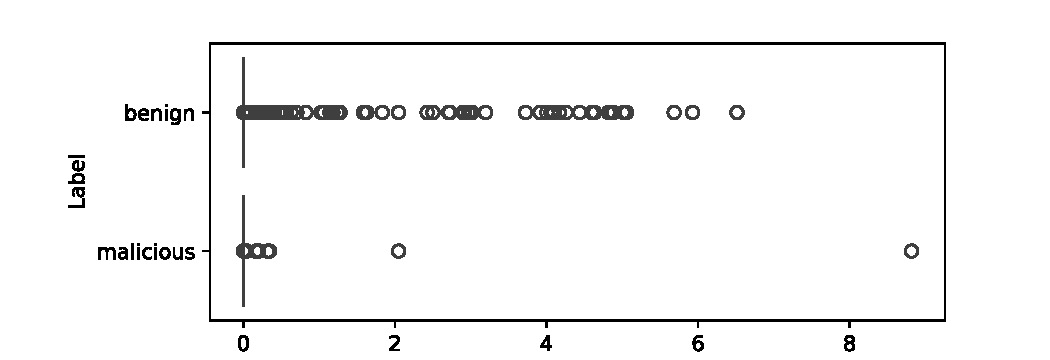
\includegraphics[width=\textwidth]{Active-Max}
      \caption{连续活跃时长最大值}
    \end{subfigure}
    ~
    \begin{subfigure}[b]{0.48\textwidth}
      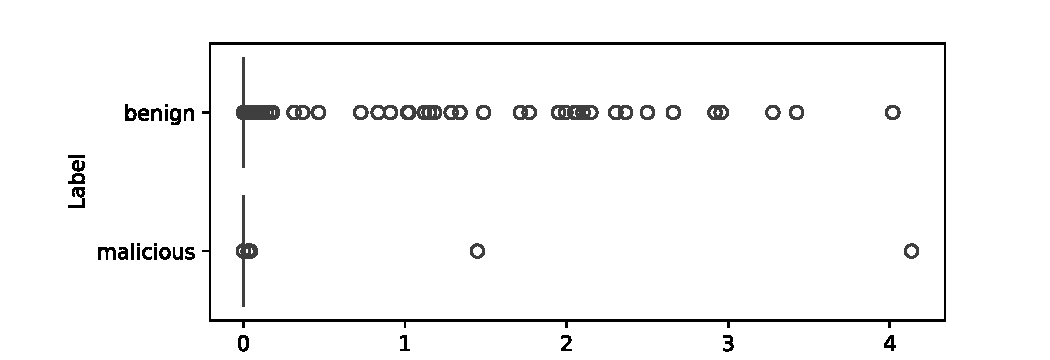
\includegraphics[width=\textwidth]{Active-Std}
      \caption{连续活跃时长标准差}
    \end{subfigure}
    \bicaption{\enspace 连续活跃时长最大值、连续活跃时长标准差箱线图}{\enspace Boxplots of active max and active std}
    \label{fig:active-max}
\end{figure}

从箱线图可以看到,网络流量在该特征下的分布呈现长尾分布,因此箱线图的箱体和线体均集中在图的左侧,几乎不可见;而图的大部分空间均被箱线图的离群点占据。实际上,网络流量在大多数特征下均呈长尾分布。

在这些离群点中,横向移动流量最右侧的离群点比良性流量更靠右,说明其连续活跃时长最大值和标准差更大。说明在集群遭受横向移动攻击后,网络的一些节点之间可能会更频繁地交换数据,这就导致了会话的连续活跃时长最大值更大,同时也带动了其标准差也跟着上升。

}

\item {批量传输类特征

在批量传输类特征中,前向每 bulk 传输字节数平均值、传输数据包数平均值和传输速率呈现出横向移动流量的值域大于良性流量的值域的特点。它们的箱线图如图~\ref{fig:bulk}~所示。

\begin{figure}[t]
    \centering
    \begin{subfigure}[b]{0.48\textwidth}
      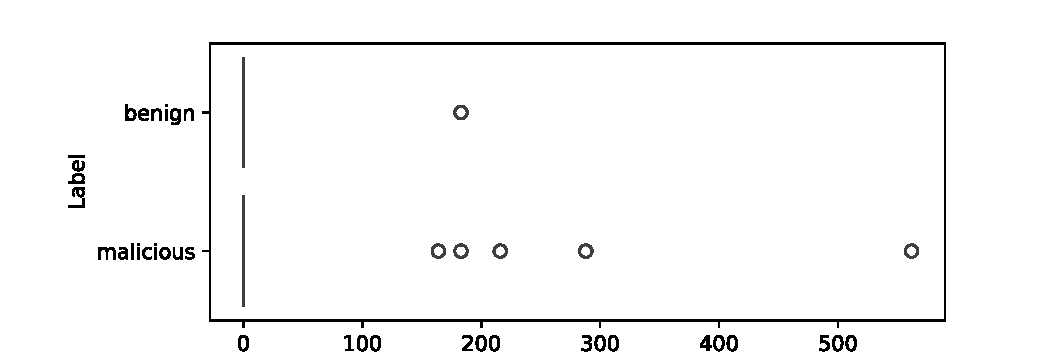
\includegraphics[width=\textwidth]{Fwd-Bytes-Bulk-Avg}
      \caption{前向每 bulk 传输字节数}
    \end{subfigure}
    ~
    \begin{subfigure}[b]{0.48\textwidth}
      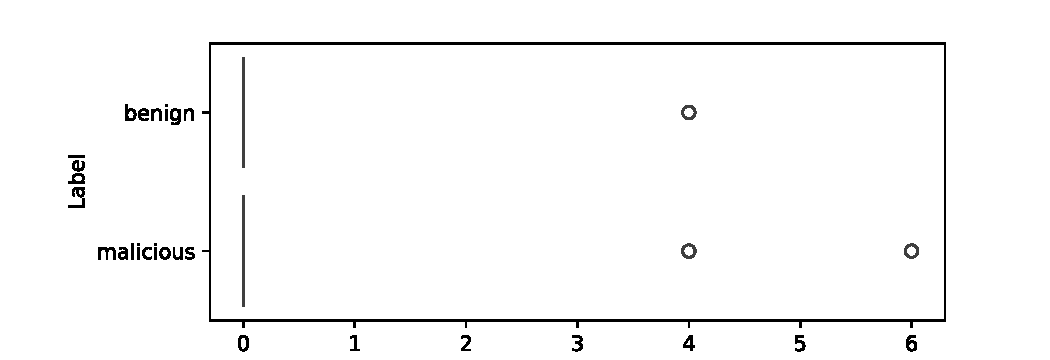
\includegraphics[width=\textwidth]{Fwd-Packet-Bulk-Avg}
      \caption{前向每 bulk 传输数据包数}
    \end{subfigure}
    \\
    \begin{subfigure}[b]{0.48\textwidth}
      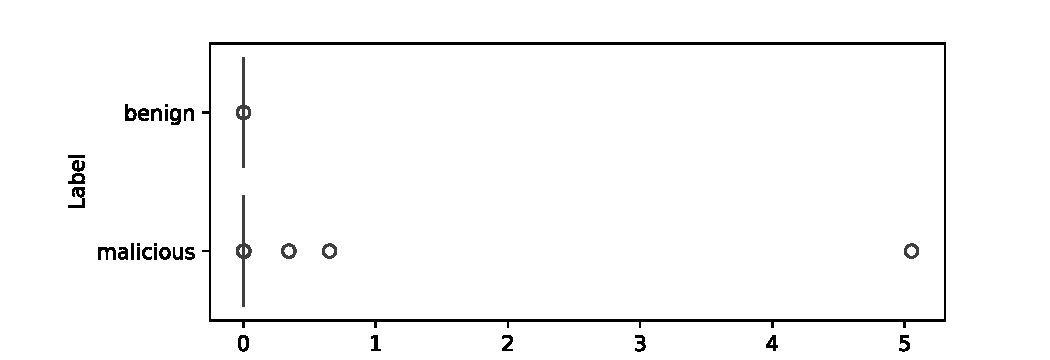
\includegraphics[width=\textwidth]{Fwd-Bulk-Rate-Avg}
      \caption{前向 bulk 传输速率}
    \end{subfigure}
    \bicaption{\enspace 前向批量传输部分特征箱线图}{\enspace Boxplots of some features of bulk data flow}
    \label{fig:bulk}
\end{figure}

结合横向移动攻击的过程,当遭受攻击的负载与攻击者的 C\&C 服务器通信,或从 API 服务器执行资源操作时,可能需要传输大量数据,以便安装恶意软件或控制集群,这会使得相应的特征的值上升。
}

\item {数据包的长度类特征

在数据包的长度类特征中,前向数据包长度最大值也可呈现出类似特点。它的箱线图如图~\ref{fig:fwd-packets-length-max}~所示。

\begin{figure}[t]
    \centering
    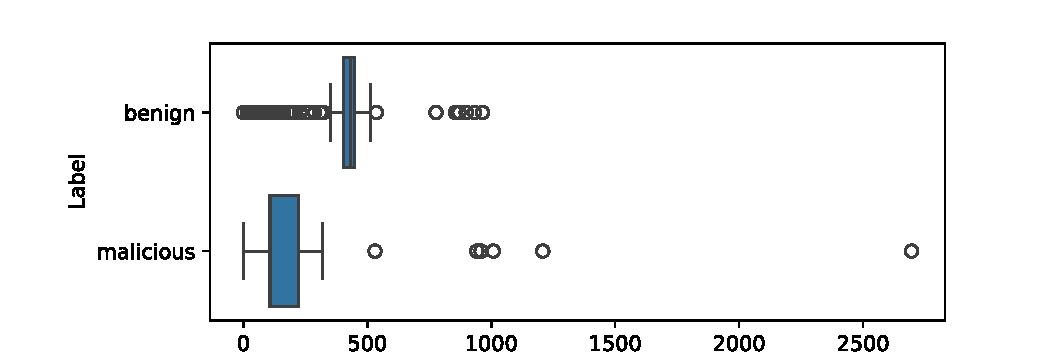
\includegraphics[width=0.48\textwidth]{Fwd-Packet-Length-Max}
    \bicaption{\enspace 前向数据包长度最大值箱线图}{\enspace Boxplot of fwd packets length max}
    \label{fig:fwd-packets-length-max}
\end{figure}
}

与上一类特征类似,结合横向移动攻击的过程,可以推断,当负载遭受攻击之后,将与攻击者的 C\&C 服务器之间传输大量数据,或向 API 服务器请求大量数据,使数据包长度的最大值上升。不过,该特征同时受到网络中最大传输单元(Maximum Transmission Unit,MTU)的影响,因此其适合与批量传输类特征一同使用,呈互补关系。

\end{itemize}

大多数特征下,横向移动流量的值域与良性流量的值域大致相同,或横向移动流量的值域小于良性流量的值域。以 IAT 平均值和前向每秒传输数据包数为例,其箱线图如图~\ref{fig:flow-iat-mean}~所示。

\begin{figure}[t]
    \centering
    \begin{subfigure}[b]{0.48\textwidth}
      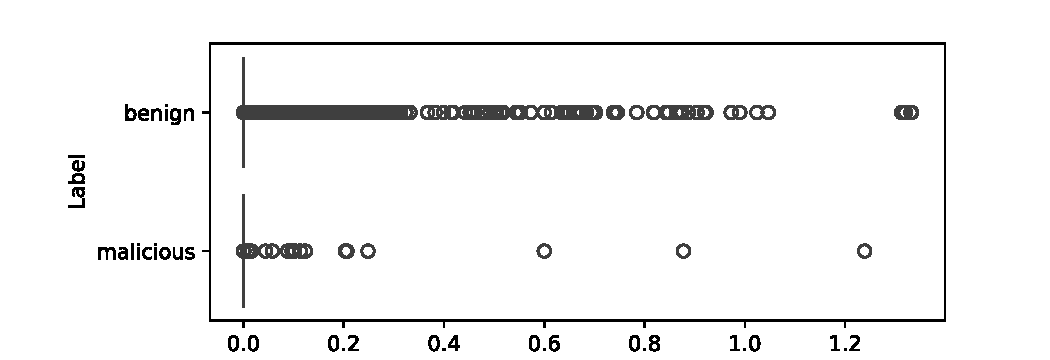
\includegraphics[width=\textwidth]{Flow-IAT-Mean}
      \caption{IAT 平均值}
    \end{subfigure}
    ~
    \begin{subfigure}[b]{0.48\textwidth}
      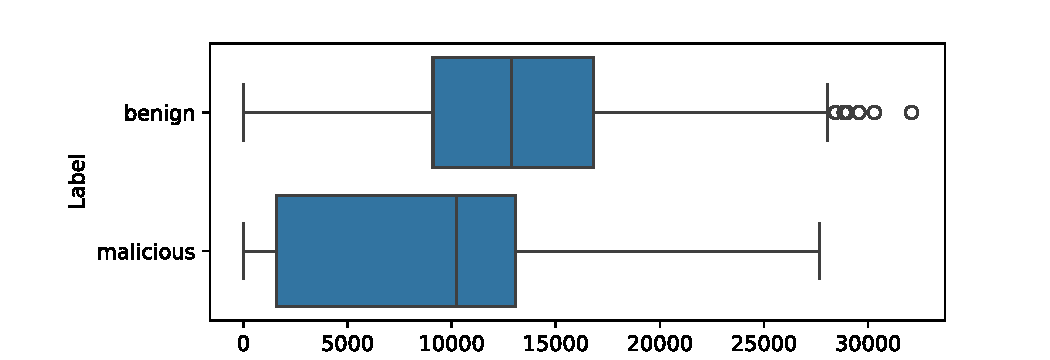
\includegraphics[width=\textwidth]{Fwd-Packets-s}
      \caption{前向每秒传输数据包数}
    \end{subfigure}
    \bicaption{\enspace IAT 平均值、前向每秒传输数据包数箱线图}{\enspace Boxplots of IAT mean and fwd packets/s}
    \label{fig:flow-iat-mean}
\end{figure}

此类特征难以区分横向移动流和良性流,因此不能直接被用来识别横向移动,需要采取机器学习等更高级的方式。

通过上述最值分析,本文发现,少量横向移动流量可以用最值法检出,这些横向移动流量代表了负载受遭受攻击之后,其与 API 服务器、与外部网络通信的流量模式发生了改变。然而,大多数横向移动流量仍不能检测出来,因此本文将进行密度分析,观察大多数流量的分布情况。

\subsection{密度分析}
\label{sec:distplots}

与箱线图相比,而直方图和密度图可以提供更全面的信息,因此,本小节将使用直方图和密度图(下文统称为分布图)进行密度分析。

虽然大多数特征呈现长尾分布,但也有少量特征不遵循长尾分布,可以不去除离群点而直接观察其分布图。这包括流速类特征、数据包的长度类特征等。

\begin{itemize}
\item {流速类特征

流速(包/秒)、前向流速(包/秒)、后向流速(包/秒)的分布图如图~\ref{fig:flow-rate}~所示。

\begin{figure}[t]
    \centering
    \begin{subfigure}[b]{0.48\textwidth}
      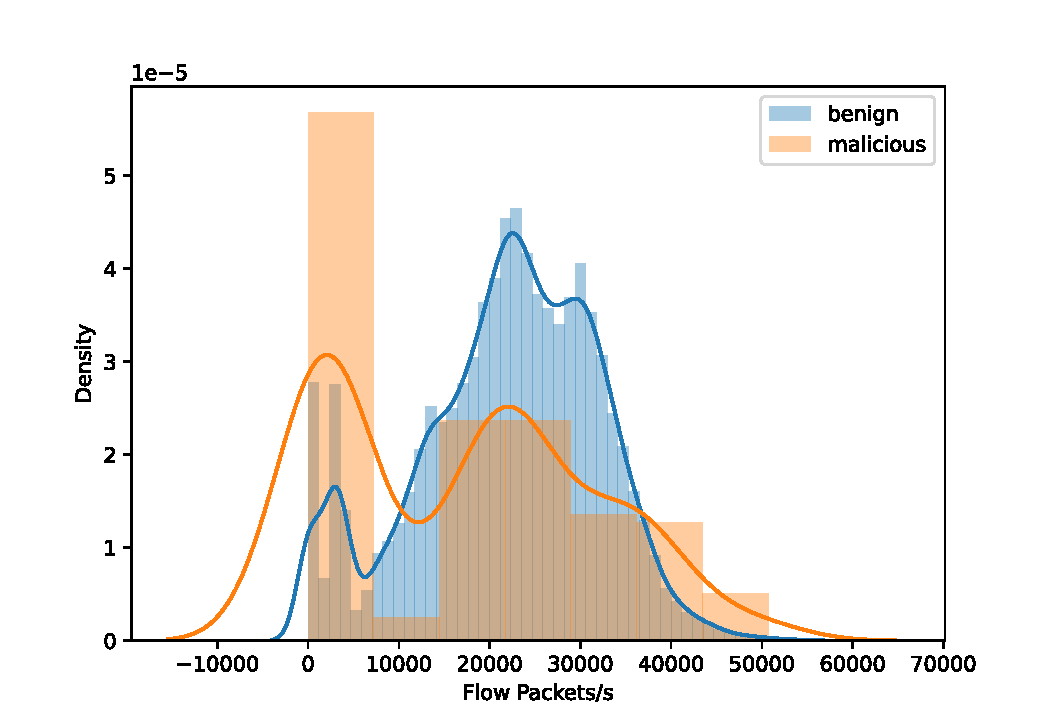
\includegraphics[width=\textwidth]{Flow-Packets-s}
      \caption{流速(包/秒)}
    \end{subfigure}
    ~
    \begin{subfigure}[b]{0.48\textwidth}
      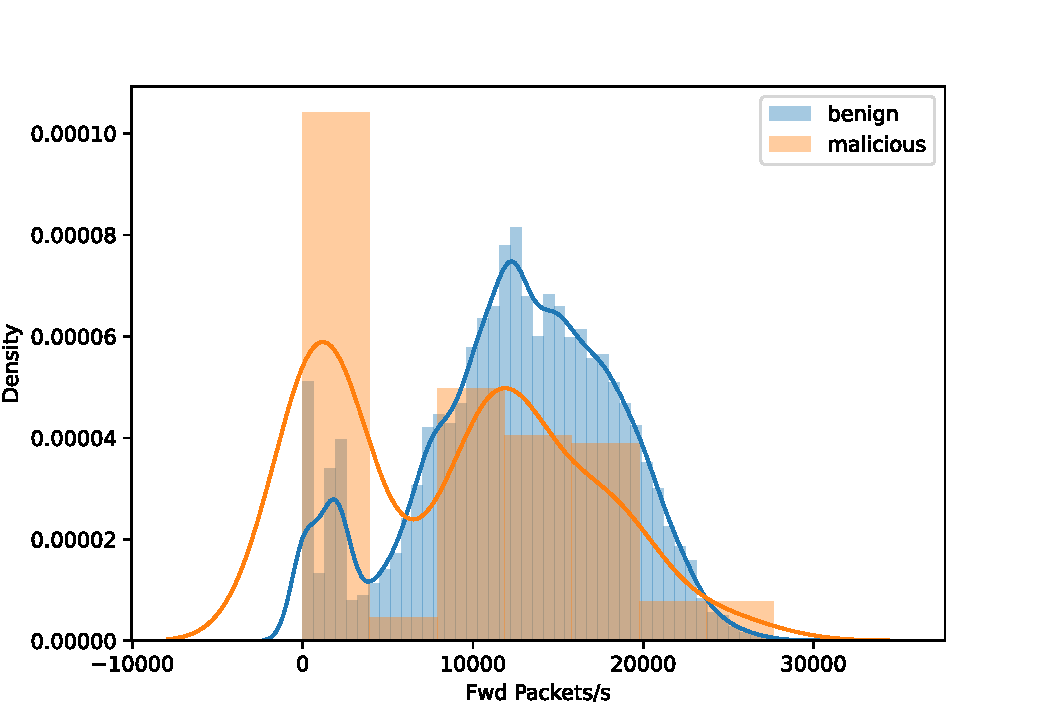
\includegraphics[width=\textwidth]{Fwd-Packets-s-1}
      \caption{前向流速(包/秒)}
    \end{subfigure}
    \\
    \begin{subfigure}[b]{0.48\textwidth}
      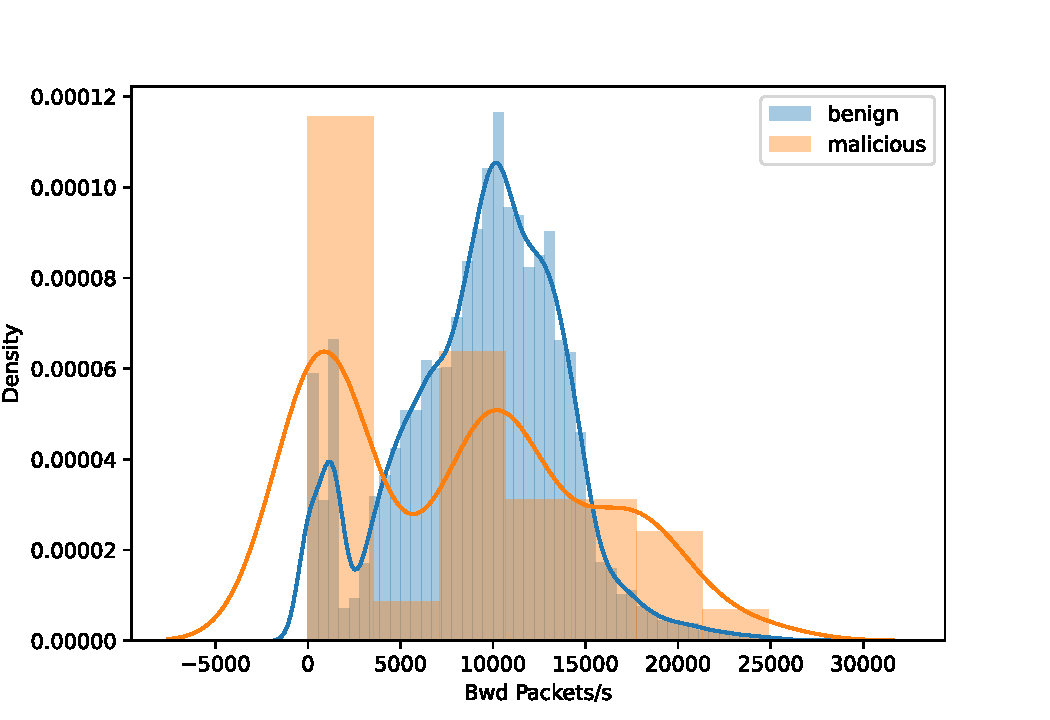
\includegraphics[width=\textwidth]{Bwd-Packets-s}
      \caption{后向流速(包/秒)}
    \end{subfigure}
    \bicaption{\enspace 流速部分特征分布图}{\enspace Distribution plots of some features of flow rate}
    \label{fig:flow-rate}
\end{figure}

横向移动流量和良性流量的流速(包/秒)、前向流速(包/秒)、后向流速(包/秒)特征均呈双峰分布,其中一峰集中于 0 附近,说明传流速慢的会话占一部分比例,这些会话可能是长连接会话;另一峰则在 10 000 至 40 000 包/秒之间,这些会话则是以数据传输为主的会话。两者的密度分布差异说明,与良性流量相比,横向移动流量的数据传输需求较低。
}

\item {数据包的长度类特征

前向数据包长度最大值、平均值、标准差的分布图如图~\ref{fig:fwd-packet-length}~所示。

\begin{figure}[t]
    \centering
    \begin{subfigure}[b]{0.48\textwidth}
      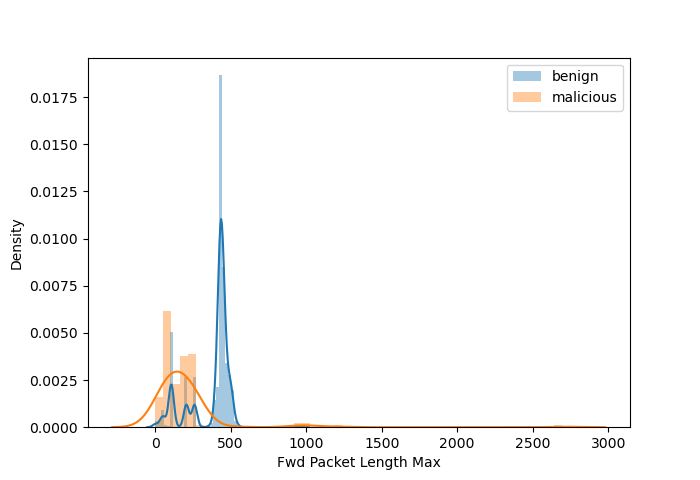
\includegraphics[width=\textwidth]{Fwd-Packet-Length-Max-1}
      \caption{前向数据包长度最大值}
    \end{subfigure}
    ~
    \begin{subfigure}[b]{0.48\textwidth}
      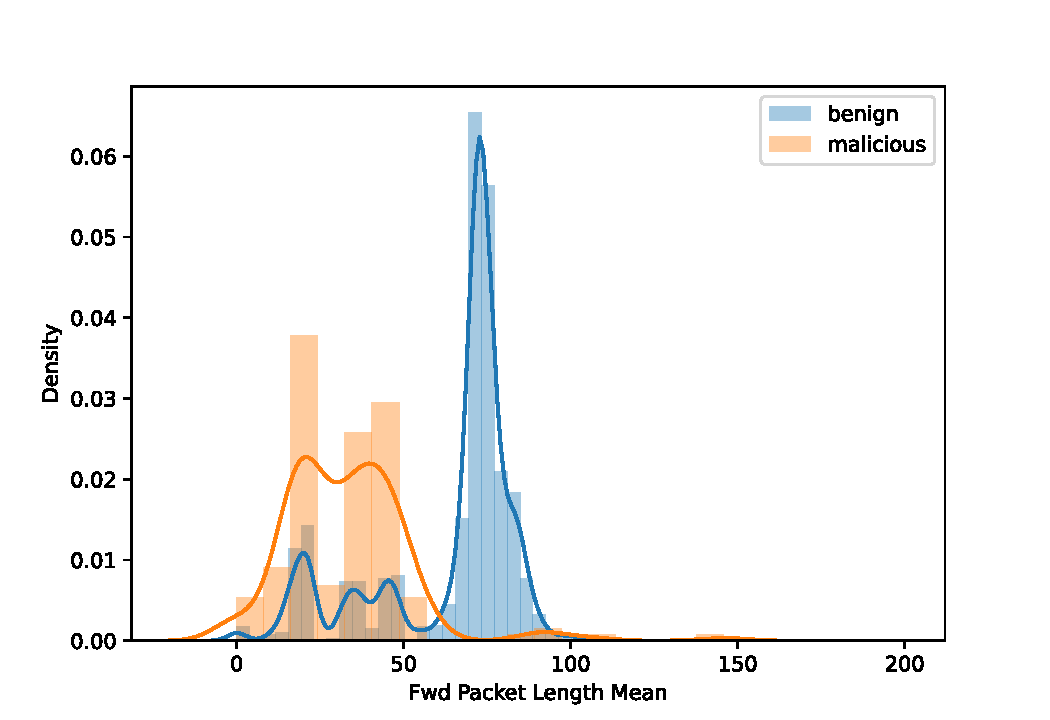
\includegraphics[width=\textwidth]{Fwd-Packet-Length-Mean}
      \caption{前向数据包长度平均值}
    \end{subfigure}
    \\
    \begin{subfigure}[b]{0.48\textwidth}
      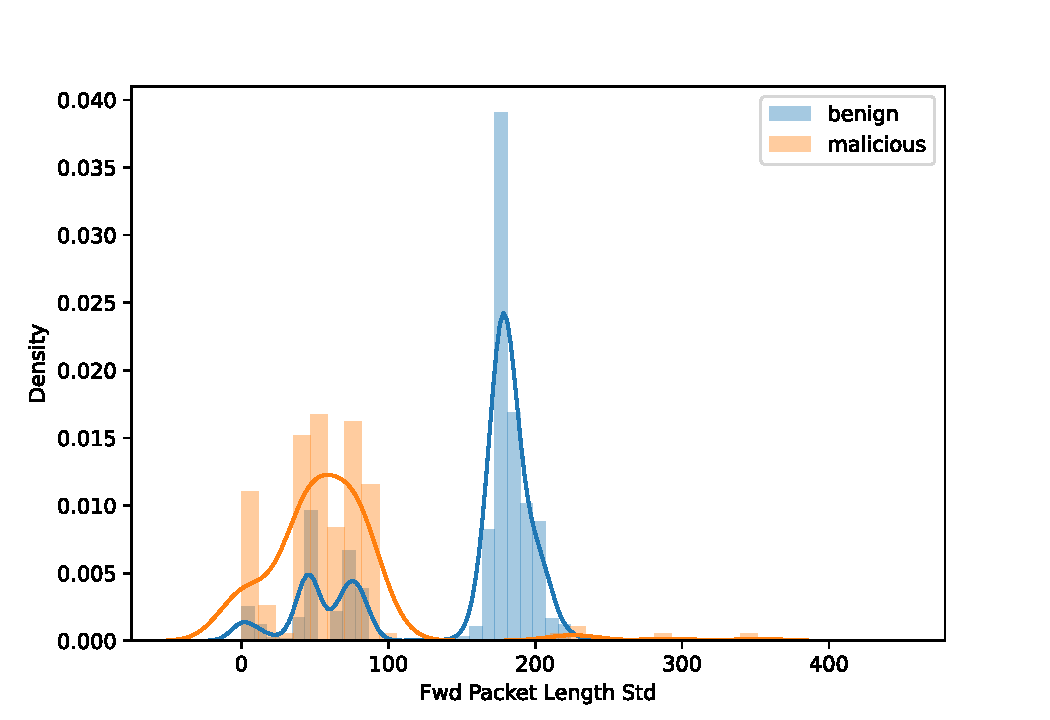
\includegraphics[width=\textwidth]{Fwd-Packet-Length-Std}
      \caption{前向数据包长度标准差}
    \end{subfigure}
    \bicaption{\enspace 前向数据包长度最大值、平均值和标准差分布图}{\enspace Distribution plots of fwd packet length max, mean and std}
    \label{fig:fwd-packet-length}
\end{figure}

横向移动流量的分布呈单峰分布,集中在 0 附近;良性流量的分布则呈双峰分布,其中一峰集中于 0 附近,另一峰则在中部。当传输大量数据时,数据包的长度较长,因此数据包长度较短时,说明此时执行的可能是简单查询操作或发起简单指令。这与 API 服务器的资源操作是匹配的。大部分横向移动流量对大量数据传输没有需求;但是,这并不排除个别横向移动流量传输大量数据的情况(见第~\ref{sec:extreme}~节)。

\item {数据包的数量类特征

在数据包的数量类特征中,后向与前向数据包比例呈现三峰分布,其分布图如图~\ref{fig:down-up-ratio}~所示。

\begin{figure}[t]
    \centering
    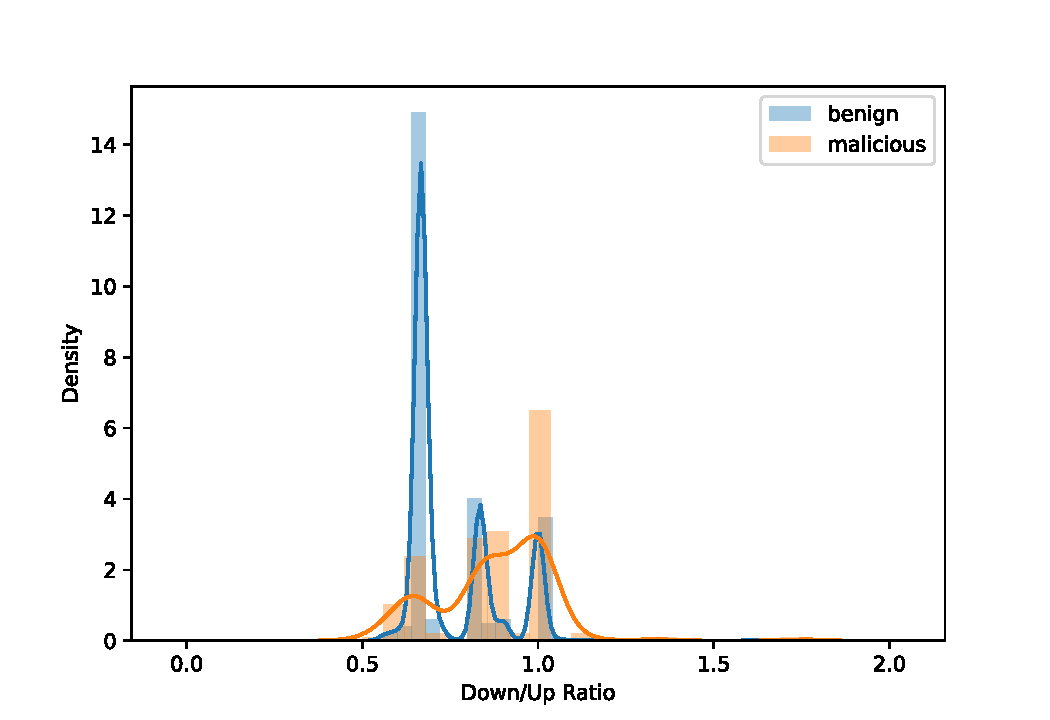
\includegraphics[width=0.48\textwidth]{Down-Up-Ratio}
    \bicaption{\enspace 后向与前向数据包比例分布图}{\enspace Distribution plot of down/up ratio}
    \label{fig:down-up-ratio}
\end{figure}

在良性流量中,大部分会话的后向数据包数量小于前向数据包,此时会话以上传为主。在 TCP 会话中,有相当一部分数据包用于维护连接,后向数据包和前向数据包数量相近,因此该比例越接近 1 时,数据包数量往往越小,说明会话中用于维护连接的数据包所占比例越大。因此,横向移动流量与良性流量的不同之处在于,横向移动流量有效传输的数据不多,它对容器化集群所提供的服务没有兴趣。
}
}
\end{itemize}

其余的大部分特征符合长尾分布,或其分布范围较窄,从分布图中难以获取有效信息。以 TCP SYN 统计和流速(字节/秒)为例,它们的分布图如图~\ref{fig:syn-flag-count}~所示。

\begin{figure}[t]
    \centering
    \begin{subfigure}[b]{0.48\textwidth}
      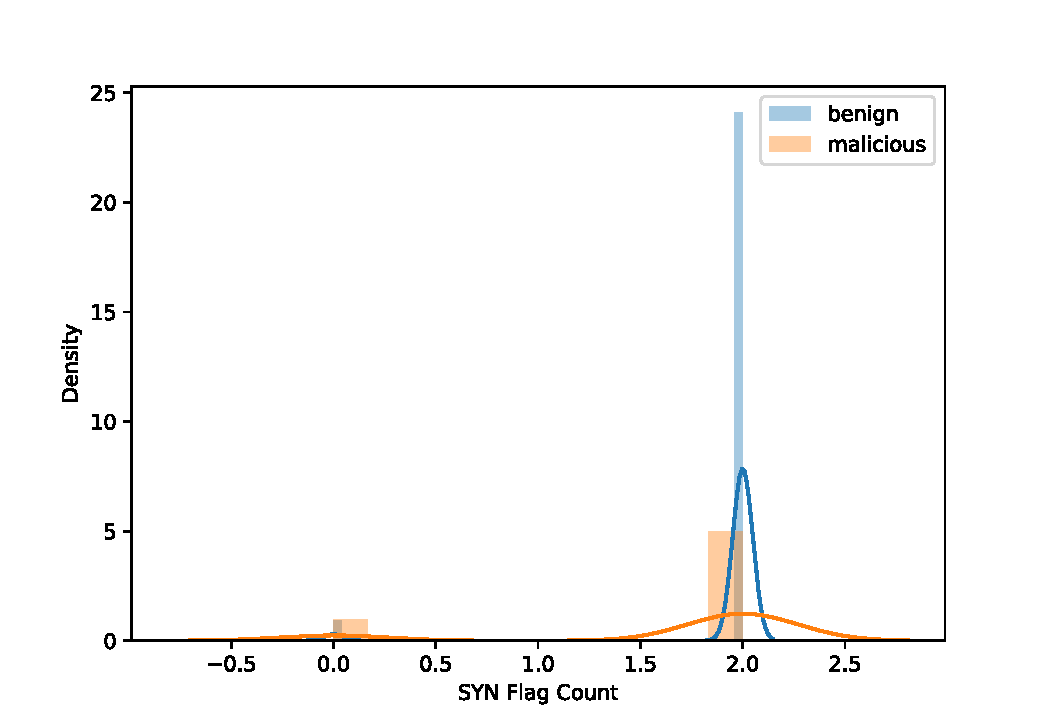
\includegraphics[width=\textwidth]{SYN-Flag-Count}
      \caption{TCP SYN 统计}
    \end{subfigure}
    ~
    \begin{subfigure}[b]{0.48\textwidth}
      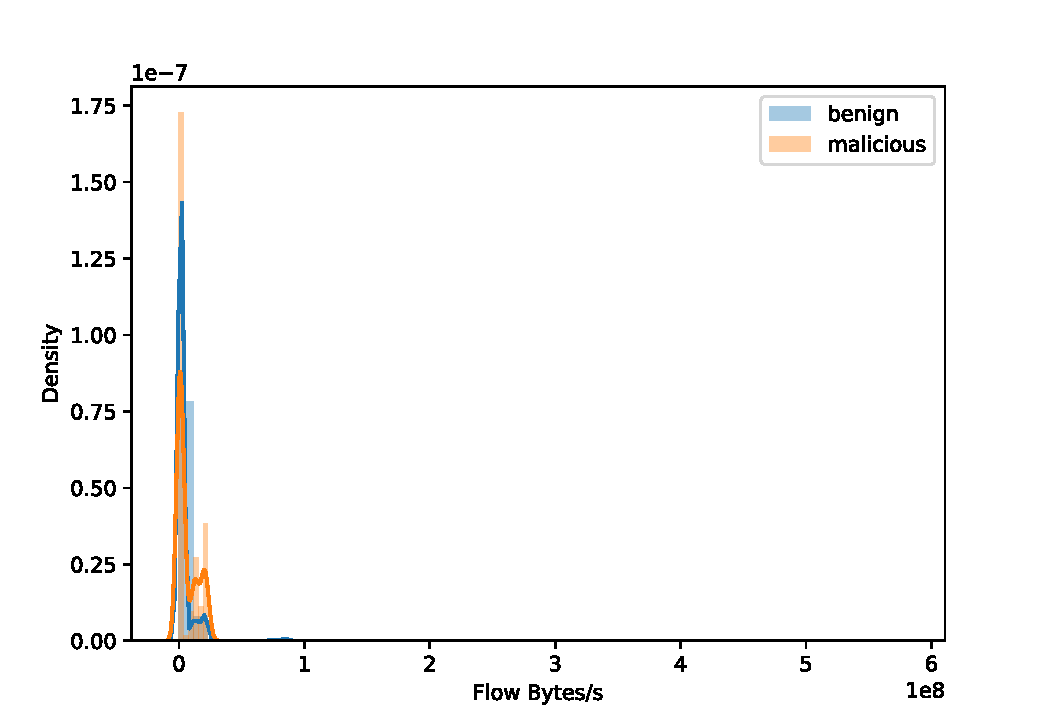
\includegraphics[width=\textwidth]{Flow-Bytes-s}
      \caption{流速(字节/秒)}
    \end{subfigure}
    \bicaption{\enspace TCP SYN 统计、流速(字节/秒)分布图}{\enspace Distribution plots of SYN flag count and flow bytes/s}
    \label{fig:syn-flag-count}
\end{figure}

\subsection{小结}

本节通过最值分析和密度分析,对横向移动流量与良性流量的差异进行了评估。通过最值分析,发现少数横向移动流量的分布超出了良性流量的范围,并且它们反映了负载遭受攻击后与 API 服务器及外部网络的访问模式发生了变化。通过密度分析,发现横向移动行为与良性流量相比,通常不需要很高的数据传输量,这使得大部分横向移动流量隐蔽在良性流量之间。此外,大部分网络流量特征呈长尾分布。因此,需要采用机器学习的方式进行特征重要度评估,进一步挖掘其中的信息。

\section{基于机器学习的网络流量特征重要度评估}
\label{sec:filter}

使用机器学习进行数值连续型特征的筛选,通常可以采用决策树方法,也可以挖掘特征与目标变量之间的关联性。

决策树由根节点、内部节点和叶子节点组成。根节点代表整个数据集,每个内部节点代表对一个特征的判断。用于分类模型时,每个叶子节点代表一个决策分数。然而,单棵决策树通常容易过拟合、准确性较低,因此通常使用多棵决策树集成学习的方法。

多棵决策树的集成学习有两种方式:

\begin{itemize}
    \item 随机森林基于装袋(bagging)方法,从训练数据中随机抽取多个子集,对每个子集训练一棵决策树,然后将其组合得到最终的预测结果。
    \item 梯度提升决策树基于提升(boosting)方法,训练多棵决策树,其中每一棵决策树训练完成后,对该树错误分类的样本给予更高的权重,以训练下一棵决策树。
\end{itemize}

为了计算特征重要度,通常采用基尼系数。它计算的是数据集中的样本属于不同类别的概率,基尼系数越大,说明数据集越不纯,即样本属于不同类别的概率越高。对集成学习中每棵决策树的相应特征的节点计算基尼系数的降低值,然后作平均,可以得出各个特征的重要度指标。

挖掘特征与目标变量之间的关联性时,对于分类问题,一般可使用卡方检验、F检验或互信息量检验。然而,卡方检验只适用于离散型特征,而网络流量的特征主要包含连续型变量,因此不适用卡方检验。F检验要求特征服从正态分布,根据第~\ref{sec:distplots}~节中的分布图,这些特征与正态分布差异较大,因此不适用F检验。互信息量检验可用于连续型特征,对特征分布没有要求,因此可以采用互信息量检验的方法。

互信息量用于评价两个随机变量之间的依赖程度,若一个随机变量已知时,另一个变量的不确定性(熵)减少,则这两个随机变量的互信息量较高。互信息的计算公式\eqref{eq:multi-info}如下:

\begin{figure}[t]
    \centering
    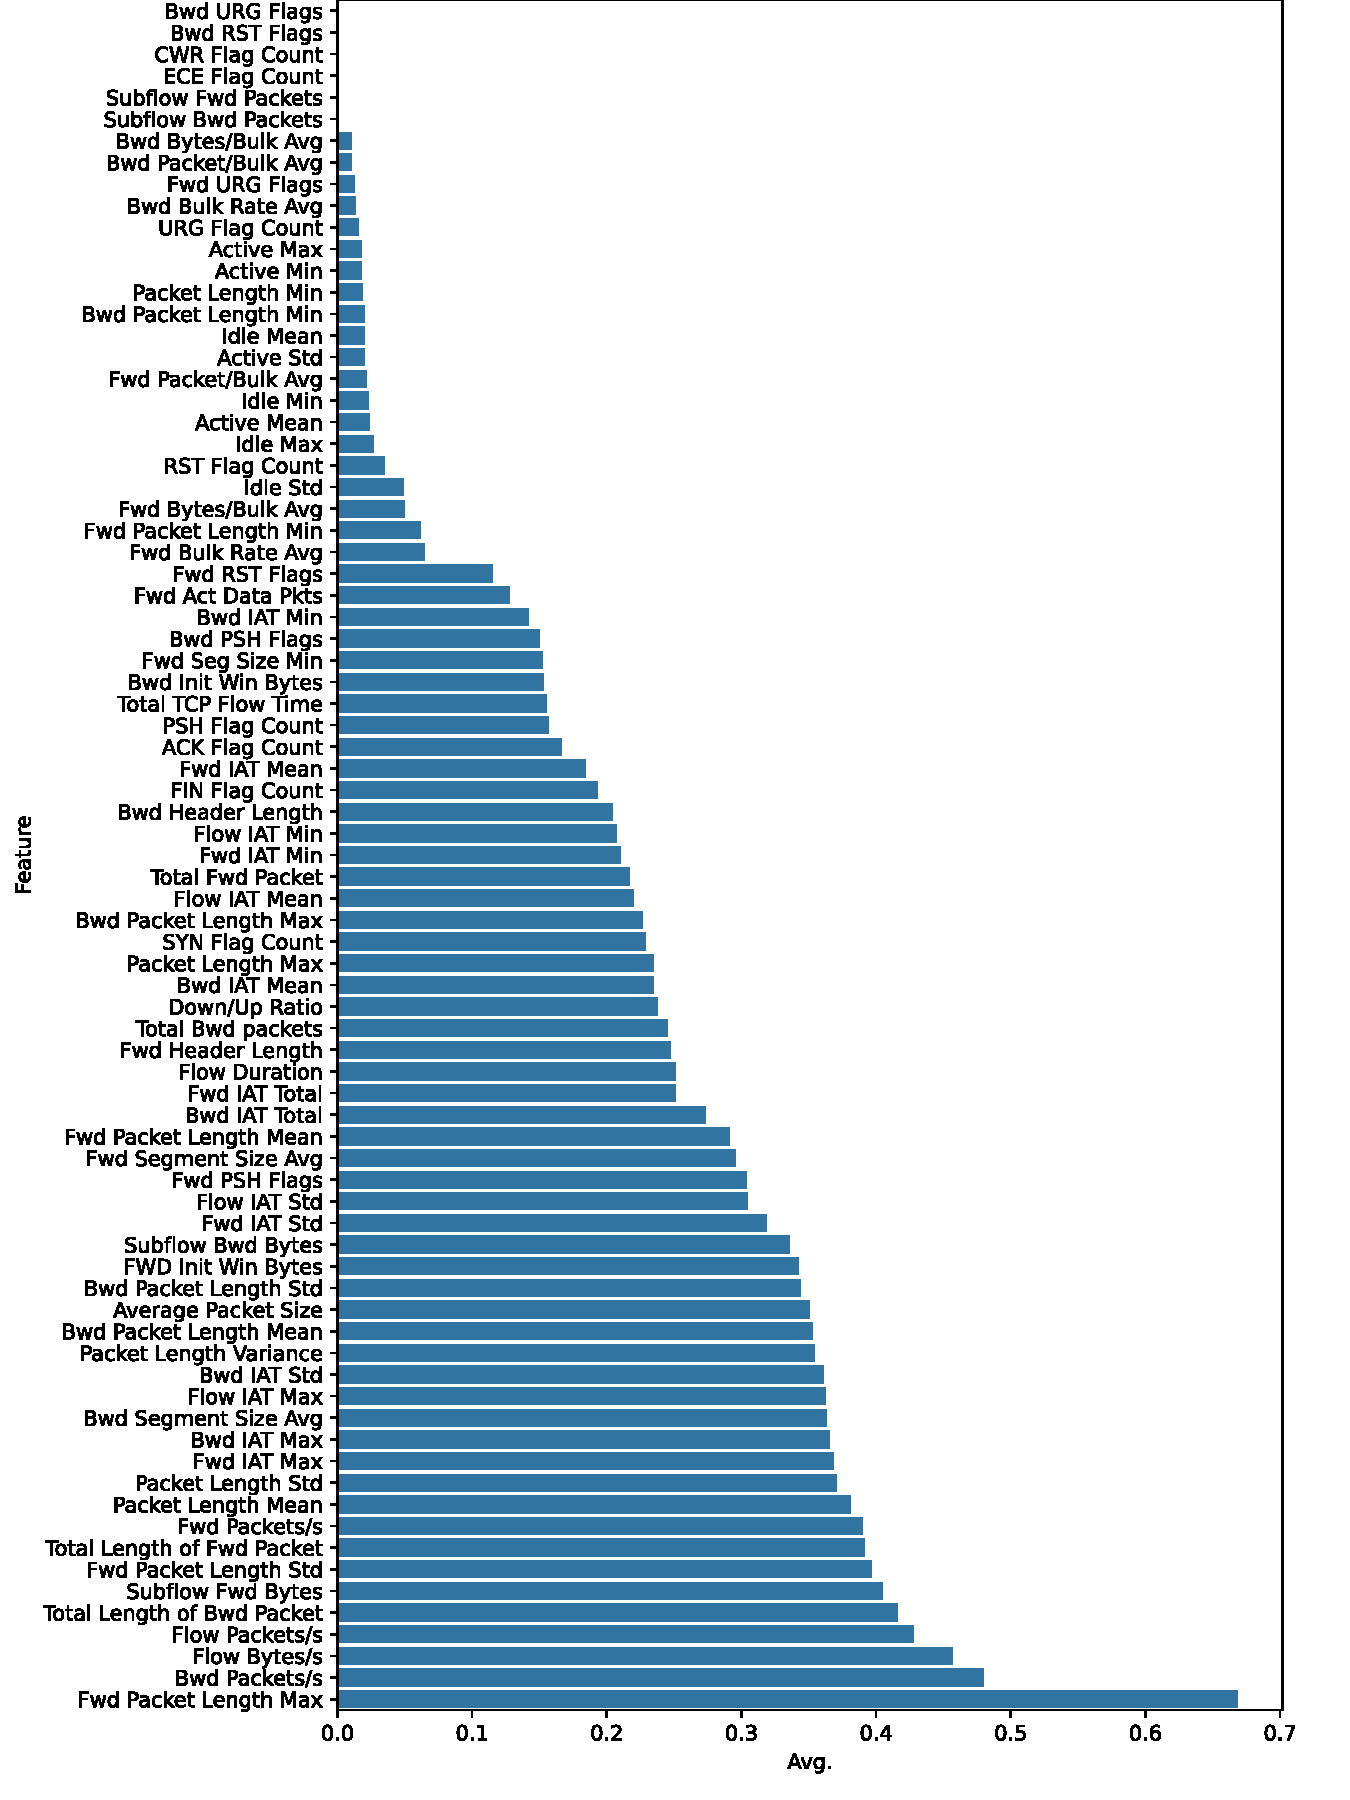
\includegraphics[width=1.0\textwidth]{unimportance}
    \bicaption{\enspace 网络流量中各特征的重要度}{\enspace The importance of features of flows}
    \label{fig:unimportance}

\end{figure}

\begin{equation}
    \label{eq:multi-info}
    \begin{split}
        I(X;Y) &= \sum_{x \in X} \sum_{y \in Y} p(x,y) \log \frac{p(x,y)}{p(x)p(y)}.
    \end{split}
\end{equation}

在公式\eqref{eq:multi-info}中,$X$ 和 $Y$ 表示两个变量,$p(x,y)$ 表示这两个变量的联合概率分布,$p(x)$、$p(y)$ 表示边缘概率分布。该公式用于计算 $X$ 和 $Y$ 的依赖程度。通过评价网络流量各特征与其标签的依赖程度,即可得到特征的重要度。

本文通过使用梯度提升决策树、随机森林、互信息量分别得到各特征的重要度,并缩放至$\left[0,1\right]$区间后,按其平均值从低到高排列,如图~\ref{fig:unimportance}~所示。

三个模型一致认为后向 URG、后向 RST、CWR、ECE、前向子流数据包数、后向子流数据包数等六个特征的重要度为零,因此可以从数据集中删除。前向数据包长度最大值的重要度最大,这也验证了第~\ref{sec:analyze}~节中的讨论。其他特征的重要度则呈梯级分布。这些特征的重要度将在后续的模型设计中得到应用。

\section{实验评估}

由于后续章节将使用基于流量预测的方法进行横向移动检测,本节将使用 GRU 模型来验证特征重要度评估方法,将最不重要的若干个特征删除,并与另一种常见的特征降维方法,主成分分析(Principal Component Analysis,PCA),进行对比。数据集和评估指标分别如第~\ref{sec:experiment-dataset}~节和第~\ref{sec:kpi}~节所述。实验对比了全量特征(79维)、筛除一部分特征(剩余57维)和使用 PCA 压缩到57维的结果,如表~\ref{tab:analyze-expreiment-result}~所示。

\begin{table}[!htbp]
    \bicaption{\enspace 特征降维方法对比实验结果}{\enspace Comparison results of feature dimensionality reduction}
    \label{tab:analyze-expreiment-result}
    \centering
    \footnotesize% fontsize
    \setlength{\tabcolsep}{4pt}% column separation
    \renewcommand{\arraystretch}{1.2}%row space 
    \begin{tabular}{ccccccccc}
        \hline
        实验项目 & 特征维度 & TPR & FPR & F1 & AUC\\
        \hline
        全量特征 & 79 & 0.7239 & 0.2814 & 0.0934 & 0.8080\\
        筛除一部分特征 & 57 & 0.7423 & 0.2543 & 0.1046 & 0.8113\\
        PCA & 57 & 0.7178 & 0.2795 & 0.0932 & 0.8038\\
        \hline
    \end{tabular}
\end{table}

结果表明,使用本文提出的方法进行降维,去除无关特征后,模型的性能有所提高,AUC 达到 0.8113,四个指标均为最优;若使用 PCA 进行降维,模型性能反而下降,并且 PCA 丢失了降维方法的可解释性。因此,本文提出的特征重要度评估方法是有效的,并且比 PCA 方法更优,后续在第~\ref{sec:feature-filter}~节还将进行进一步验证。

\section{本章小结}

本章首先对横向移动原理进行分析,指出了横向移动将导致容器化集群中的负载、主机和 API 服务器的流量模式发生改变。接着,本文通过特征分析,指出了这种改变主要存在于两个方面:对于少量但是关键的横向移动流量而言,它会传输大量数据,导致部分批量传输特征、数据包长度特征的值超出了良性流量的值域,这是因为负载处在攻击者的 C\&C 服务器的控制之下,攻击者在负载上安装恶意软件或脚本,并从 API 服务器窃取关键信息;对于大部分横向移动流量而言,它们的特征分布与良性流量也有所差异,横向移动往往具有更低的数据传输需求。最后,本文通过基于决策树和互信息量检验的特征重要度评估,验证了特征分析的结论,并得到了各特征的评估分数,这将在后续的模型设计中得到应用。
}